\documentclass{report}
\usepackage{graphicx}
\usepackage[hidelinks]{hyperref}
\usepackage{cite}
\usepackage{appendix}
\usepackage{pdfpages}
\begin{document}
\begin{titlepage}
    \begin{center}
        \vspace{1.0cm}
        
\includegraphics[scale=0.5]{Warwick}
        \vspace*{1cm}
  
        % Title
        \textbf{Using Ad Hoc Networking in Emergency Situations}
  
        \vspace{0.5cm}
        % Subtitle
        Spreading information in an emergency situation to help both people in danger and the emergency services
  
        \vspace{1.5cm}

        % What the project is about
        \textbf{Project Specification}
  
        \vspace{1.6cm}

        % Author name
        \textbf{Freddie Brown}\\
        \textbf{u1716717}


  
        \vspace{1.6cm}
        % Information about the institution
        Supervisor: Dr. Matthew Leeke\\
        Department of Computer Science\\
        University of Warwick\\
        2019-20
  
    \end{center}
\end{titlepage}


\chapter*{Abstract}
\pagenumbering{roman}
\addcontentsline{toc}{chapter}{Abstract}

During a disaster, it is often very difficult to communicate using our devices. Whether this be because 
infrastructure has been damaged, or there is too much traffic over networks. This can mean people feel 
isolated and makes it difficult for the emergency services to know the situation on the ground. This 
project aims to help ease this by creating emergency Ad-Hoc networks during times of emergency. Using 
hardware already found in the devices people carry around with them day-to-day, information can be 
passed from person to person and can be sent to the emergency services. It could help improve the efforts of the emergency services by giving them a better picture of an area, helping to use their resources more effectively. This lets them to save more lives.
\\
\\
\textit{Keywords: Bluetooth, Ad Hoc, MANET, Emergency, Disaster}


% \chapter*{Acknowledgements}
% \addcontentsline{toc}{chapter}{Acknowledgements}
% Acknowledgements

\chapter*{Abbreviations}
\addcontentsline{toc}{chapter}{Abbreviations}

\textbf{MANET} - Mobile Ad Hoc Network\\
\textbf{VM} - Virtual Machine\\
\textbf{BCS} - British Computing Society\\
\textbf{WSN} - Wireless Sensor Network\\
\textbf{AODV} - Ad-Hoc On-Demand Distance Vector\\
\textbf{DTN} - Delay Tolerant Network\\
\textbf{DAG} - Directed Acyclic Graph\\



\tableofcontents{}     

\chapter{Introduction}
\pagenumbering{arabic}
This project is about investigating the application of MANETs for use in emergency situations. This is a technology which lends itself to the low infrastructure needs of a disaster scenario. They can form networks dynamically with low overheads. As mentioned in the specification, these are very interesting in fluid situations where nodes move in and out of a network\cite{sun2001mobile}. Although this is the main area of exploration for the project, there are other areas which are just as important which also need to be considered. A project such as this brings up issues such as data privacy, packet routing and taking actions to prolong the battery life of a device. These are all areas which will have a huge impact on the success of a project such as this.  

\section{Motivations}
The modern world is highly connected through our telecommunications systems. These are used to connect people together. One important usage of this, is to quickly contact the emergency services. As discussed in the specification, during a disaster, such as the one seen in the 2017 hurricane in Puerto Rico, not having access to a form of communication can cause great harm to peoples lives. A study estimates that the lack of communications services in the aftermath of the hurricane contributed to an increase in mortality of 62\% \cite{kishore2018mortality}. Remote areas were hurt most, being without cellular data services for up to 41 days. It can make it difficult for rescuers to know what is going on and how to intervene such that they can make a difference. This commonly leads to high cost and disruption. Also mentioned in the specification was Hurricane Katrina, in this scenario, high winds destroyed antennas highly damaged or destroyed \cite{banipal2006strategic}, many of which belonged to belonged to cellular providers.
\bigskip\\
This illustrates the need to develop systems which help to ensure connectivity, even in challenging times. The United Nations voted, in June 2016, that internet access is a human right that should be protected \cite{UNResolutionJune2016}. This puts our current systems under the microscope and shows how important these services are to people and how access to them can save lives.  

\section{Project Aims}
This project is aiming to develop a system which could be integrated into future mobile devices, which allows for the dissemination of emergency information in the event of a disaster. The project will look at the different ways which this can be implemented, what the challenges are that this problem presents as well as peripheral issues which were mentioned earlier.  

\section{Stakeholders}
As mentioned in the specification, the stakeholders in this project are those which will benefit from a system such as this being implemented. Those who live in areas which are frequently affected by large scale emergencies will be the ones who will use this more often. Furthermore, the emergency services will benefit greatly from a project like this so they can maintain a clearer picture of what the situation on the ground its, and where their efforts will be most effectively utilised.  

\chapter{Research}

\section{Related Work}
Emergency networks are difficult to implement because of, in many cases, the damage to infrastructure that is caused in an emergency or the strain that puts on the existing infrastructure. Disasters can be difficult to deal with after they happen due to this degradation in communications infrastructure \cite{nprDorian}. This can then hamper efforts to rescue survivors as they will struggle to communicate with those who need saving. Having a system in place, specially for this scenario, could save the lives of those that are affected by disaster \cite{sciAmHurr}. 
\bigskip\\
An interesting attempt to solve this problem is HIRO-NET\cite{ferranti2019hiro}. This system has 2 tiers: a local meshing using Bluetooth Low Energy (BLE) to connect devices together using a client-server model, and a way to connect together these local networks. In local meshing, a node starts off as a client and will try and find a server to connect to. After a while, it will timeout and will become a server for nodes to connect to. Doing this means that, when nodes join to network, over time it becomes easier to connections to form. Piconets are joined together to form Scatternets and packets are transported within them. If a Piconet has an active internet connection, the server will declare this. This means that other servers will route packets to this Piconet to be sent out over the active connection. This system is complex but allows for a more regular level of service for users.
\bigskip\\
A more simple approach then HIRO-NET has a greater focus on providing information for the emergency services\cite{wu2011emergency, shahin2015alert}. It takes some information, such as geographical information, and transports it to a central node to allow this information to be aggregated. The suggested systems use both WiFi and Bluetooth and how they can both play an important role together. These conclude that, as WiFi has a wider range and is more available, it plays a more important roles than Bluetooth. It also states that using WiFi Direct can provide a large speed boost when spreading information\cite{shahin2015alert}. It means that a connection doesn't need to happen for a device to spread critical information about itself, which has obvious benefits for the types of situations that this project is investigating. 
\bigskip\\
WiFi is an incredibly important technology as it supports long range transmission. For some standards, transmission can be up to, or close to, 1,000m in certain situations \cite{sun2013ieee, abdelgader2014physical}. Bluetooth tends to be used more for short range transmissions \cite{bhagwat2001bluetooth}. It relies on being in quite a well populated area as its range is limited. Each have their uses. Bluetooth is also considered to be more power efficient\cite{putra2017comparison} than WiFi, but this is disputed for certain use cases \cite{friedman2012power}. This means it is sensible to consider both technologies for this project. This project is focusing on close range communications in environments where users may not have access to a stable power source. For this reason, Bluetooth may be a better choice than WiFi. WSN systems which use Bluetooth could provide an ideal model to analyse, such as \cite{chu2010design}. This example discusses a high performance sensor network using highly optimised hardware. It presents an interesting model for nodes to work efficiently, such as only have 1 outgoing route for traffic. This could be applied in this project by only allowing a node to send data to 1 other node at any point. 
\bigskip\\
A more recent, and very applicable, example of Ad Hoc networks is in the automotive industry. As cars have become more advanced, they have included more powerful computers on-board. Research has been done which looks into how they can be used to form networks made up of these vehicles. A number of studies \cite{zheng2016cooperative, kaur2017analysis, hu2017performance} have investigated different aspects of this type of network. As discussed in \cite{zheng2016cooperative}, VANETs can communicate with each other as they drive past each other, communicating information between themselves. This information could be about similar things to the data in this project, such as location data of interesting events, like traffic jams. Although, as also discussed in \cite{zheng2016cooperative}, this isn't a stable network as they may be moving too fast to be able to communicate effectively. It offers a number of solutions, such as using store-and-forward routing algorithms or using Cellular data. VANETs also have a number of other issues similar to this project,security and routing. \cite{hu2017performance, kaur2017analysis} discuss a number of different possibilities for routing, such as novel ideas like geographical routing\cite{hu2017performance} and more established routing protocols such as AODV \cite{perkins1999ad, kaur2017analysis} and how well they perform in this paradigm.

\section{Security}

Security is an area of this project which needs serious consideration. The legal and social ramifications \cite{bbcData} of ignoring it can be extremely high. As this project is dealing with sensitive location data, it is crucial that a solution is found that will ensure integrity and confidentiality. If it isn\'t, data could be harvested and used to the detriment of those who survive a disaster. An example of post--disaster problems is looting, which was seen after Hurricane Katrina in 2005\cite{nbcKatrina}.
\bigskip\\
Firstly, a method of sharing a key with the nodes is needed so they can encrypt information before it is transmitted. A way to accomplish this is to use Diffie--Hellman key exchange\cite{diffie1976new} so symmetric key encryption may be used. As suggested by \cite{li2010research}, this protocol has issues with security and is susceptible to man in the middle attacks. 
\bigskip\\
An alternative to using symmetric key encryption is using public key encryption, such as RSA \cite{aufa2018security}. In this, each member which wants to receive data will declare their public key, which is available to everybody. Once the message has been encrypted with the public key, only the private key can decrypt the message. As the private key should only be known by 1 users, this means only the correct recipient may view the encrypted data. This will provide messages with the confidentiality that is needed. 
To provide integrity to the messages, digital certificates could be used \cite{diffie1976new}. 

\section{Routing}
As Bluetooth uses a client-server model, routing is usually device-to-device. With this, it forms multiple small groups of devices (Piconets). These can be joined together and packets can be routed between them. Furthermore, other topologies which aren't as stable also exist, and so packet routing needs to be investigated in these forms too. By investigating all of these, a variety of circumstances can be covered. 
\bigskip\\
As MANETs are already in use in a variety of situations, there are a couple of routing protocols that are already used. One popular one is AODV \cite{phong2010enhancing, perkins1999ad}, a combination of dynamic source routing and distance vector routing. This algorithm uses a series of packets to build routes, which are stored in nodes throughout the network. These are built using Route Request(RREQ) packets being broadcast across the network, flooding it. When an RREQ packet reaches the desired node, a Route Reply (RREP) packet is broadcast back, along the path which was used to reach the node in the first place. When an RREP packet is received by a packet which transmitted an RREQ packet, it creates a pointer in its routing table. This means it knows where to route any packets for that node in the future. 
\bigskip\\
Another algorithm which is used for routing within MANETs is TORA \cite{park1997highly}, a type of routing algorithm that uses a DAG to determine which nodes to route packets through to the destination of the packet. If a node wants to route packets to a sink, F, it will broadcast QRY packets, which are relayed until it reaches a node adjacent to F. When it reaches these nodes, they broadcast a UPD packet which contains the id and distance from the sink node. These are propagated back towards the source node. This allows a graph to be constructed and allows routing to be done based on distance. The advantage of this method is that it has fewer control packets compared to other, similar methods as it only reacts when changes are discovered in the topology. Furthermore, partitions in the network are easily detected, whereas in AODV the source will send lots of RR packets which will flood the network.    
\bigskip\\
An interesting are of packet routing, is swarm-based packet routing. It has been shown to perform better than a number of other, more established routing algorithms \cite{lin2014performance}. Swarm-based algorithms tend to find the best path in a network, but also include a probability that a different route will be chosen. As a MANET is an inherently unstable network, this is good as it allows new, better paths to be found. It also includes a time parameter to force information to be recalculated if it hasn't be used in a while. This feature also forces the exploration of new, quicker paths in the network. This type of routing is typical of a number of swarm-based routing algorithms, such as ant-colony routing\cite{sharvani2009different}.
\bigskip\\
An alternative type of biological routing is based on bees\cite{leonov2016modeling}. This protocol has a scouting stage where each node in the network is \'scouted\'. Scout packets will be sent out to each neighbour and will travel through the whole network. They are passed on each time they visit a node until they reach a sink node. A back bee packet is then sent from this node towards the source. This process is done to evaluate the efficiency of routes between nodes. This is similar to the way that more established algorithms, such as AODV, work, except the scouting it much wider ranging, whereas in AODV, the equivalent stage is only done for 1 node at a time. This is a promising solution for MANETS, but the packet overhead might be too much for some time-sensitive cases. 
\bigskip\\
The algorithms investigated already all look at algorithms which are only really useful in networks which are more stable. Connections are broken infrequently meaning the optimisations which have been discussed, can actually make a difference. Another form of routing caters more for networks which are less stable. Optimistic routing algorithms are common in DTNs and are good spreading information quickly. There are many different examples of this. One example of this is inspired by epidemiology to model how packets can flow through a network \cite{choksatid2016efficient, de2014modeling}. It works by a node passing any information it has onto available neighbours. This is similar to how a disease might spread within a general population. Each node which receives these messages will store them and then carry them forward. If these nodes are physically moving, it allows packets to achieve large multi-hop movements with far fewer exchanges. 
\bigskip\\
An alternative to disease-based routing, is to consider another type of routing also used within in DTNs, social-based routing\cite{zhu2012survey}. This kind of routing considers the behaviours of nodes within a network. This will help improve the choices that a node makes as it considers the likelihood that the other node will forward the packets that it is going to transmit. It uses a group of set social characteristics to determine whether its behaviour is 'good' and cooperative or if its 'bad' and only caring about its own resources e.g only forwarding on messages from a select group of users. Other studies, such as \cite{wong2015performance, zhu2013relative}, show how powerful social-based routing protocols can be. They help to reduce the number of packets which are sent, and increase the probability that these packets actually are delivered. As can be seen in \cite{zhu2013relative}, the chance of delivery is lower than epidemic routing, but the number of packets which are sent is far lower and the latency is far greater. This could help to reduce traffic and unnecessary traffic in the network.

\chapter{Ethical, Social, Legal and Professional Issues}

\section{Ethical Issues}

Ethical issues can come up when a project has a number of different objectives, each with negative effects which aren't immediately present. The benefits this objective could bring, if fulfilled, might out weight the immediate negatives for an objective and so due diligence on other impacts may be forgone. An example of this is in a project which collects lots of personal data. An objective of the product might be to increase cash flow of the company. Using this data to provide products such as targeted adverts may seen like a good idea at first, but might create some reputations damage in the long run. These kinds of issues may lead to data leaking or some people may find this an invasion of privacy. These damage had impacted Facebook recently. \cite{fbbreak}. In this project, location data is used among a number of nodes. This data should be protected so that it can't be used for anything unintended by nodes which have access to it. This could be through encryption or forms of providing data privacy. 

\section{Social Issues}

Social issues are those that have an affect on the lives of groups of people. As discussed in the project specification, these problems could affect how people interact with each other or could limit their access to certain goods and services. It may also relate to certain groups having access to key services over other, marginalised groups. It is difficult to see any of these issues relating to this project but this should be continually reviewed as the project moves onwards. 

\section{Legal Issues}

A large part of this project is about sending sensitive data about vulnerable people, issues around data privacy need to be considered seriously. In this project, data is being sent to other devices nearby, so trust issues which may arise. To counter this, encryption could be used to provide data privacy. By doing this, it limits access only to users who should have access to the data. Otherwise, if this isn't protected, malevolent users may use it to cause harm to others, such as terrorists looking to find people to harm. 

\section{Professional Issues}

As mentioned in the project specification, the project will adhere to the BCS Code of Conduct \cite{BCSCoP}. The aim of the project is to produce a research project which can be used in the future. This means adhering to these rules is very important. Furthermore, the project will pay close attention to the Research Code of Practice at the University of Warwick \cite{UniWarwickCOP} and the departmental rules on ethical consent for any data the project may collect from participants in any potential testing \cite{WarwickEthics}. 

\chapter{Project Requirements}

\section{Functional}

\textbf{FR1} - The system must use a widely used MAC layer protocol such as Bluetooth or WiFi.\\
$\newline$
\textbf{FR2} - The system must use data privacy techniques, such as encryption, to prevent data falling into the wrong hands. \\
$\newline$
\textbf{FR3} - The system could monitor battery life and make choices based on its predicted life expectancy\\
$\newline$
\textbf{FR4} - The system could use a system of authentication to verify nodes, such as using a trust-based system or digital certificates\\
$\newline$
\textbf{FR5} - The system must use the concept of sources and sinks, where sinks collect data and don't transmit information packets, and sources send and receive information from other sources. \\
$\newline$
\textbf{FR6} - System must have a way to identify devices within the network. This ID should be used within packets sent by each device about themselves.\\
$\newline$
\textbf{FR7} - Project could use a location discovery service such as GPS to get location data\\
$\newline$
$\newline$
$\newline$


\section{Non-Functional}

\textbf{NFR1} - The system must be fully documented and maintainable. This means that the project is easily extensible and can easily be implemented on other platforms.\\
$\newline$
\textbf{NFR2} - The system must be easy for a user to connect to and use. This is vital for the project as time is an important factor in an emergency situation and so the less time a user has to worry about how it works, the quicker they can use it to get help\\
$\newline$
\textbf{NFR3} - The system must be created so it can be applied to a large population of devices. This project works optimally if there are a large number of devices to connect so design choices should consider the need for this project to work at a large scale.\\
$\newline$
\textbf{NFR4} - The system must be able to be used by different types of devices such as Phones, Tablets and PCs. Much like \textbf{NFR3}, this project should be designed so it can be easily transported onto other devices so that they can also participate.\\
$\newline$
\textbf{NFR5} - The system must use secure communications so bad actors cannot steal and weaponise the information. \\
$\newline$
\textbf{NFR6} - System should require as little user interaction as possible to increase efficiency.\\


\section{Constraints}

As was discussed in the project specification, the project is constrained by the number of devices which it can be tested with. It is very expensive to test on a number of devices so, for that reason, the project will use a cheaper alternative, the Raspberry Pi. This will demonstrate the applications of this project, but can't replicate a proper use case of this project as it will lack the scale of devices which would be needed.
\bigskip\\
Another constraint is the types of devices, that can be used. The research will focus on applications in a heterogenous network of devices but it is likely this will only be demonstrated on a homogenous network as more popular devices (e.g iOS and Android\cite{mobileOS}), which this type of system would be employed on in the real world, require separate development. This is outside of the scope of this project as it would require more time than is available to it. This would be a stretch goal for the project or could be considered a further extension for the future.

\chapter{Project Management}

\section{Project Timeline}
\begin{figure}
    \centering
    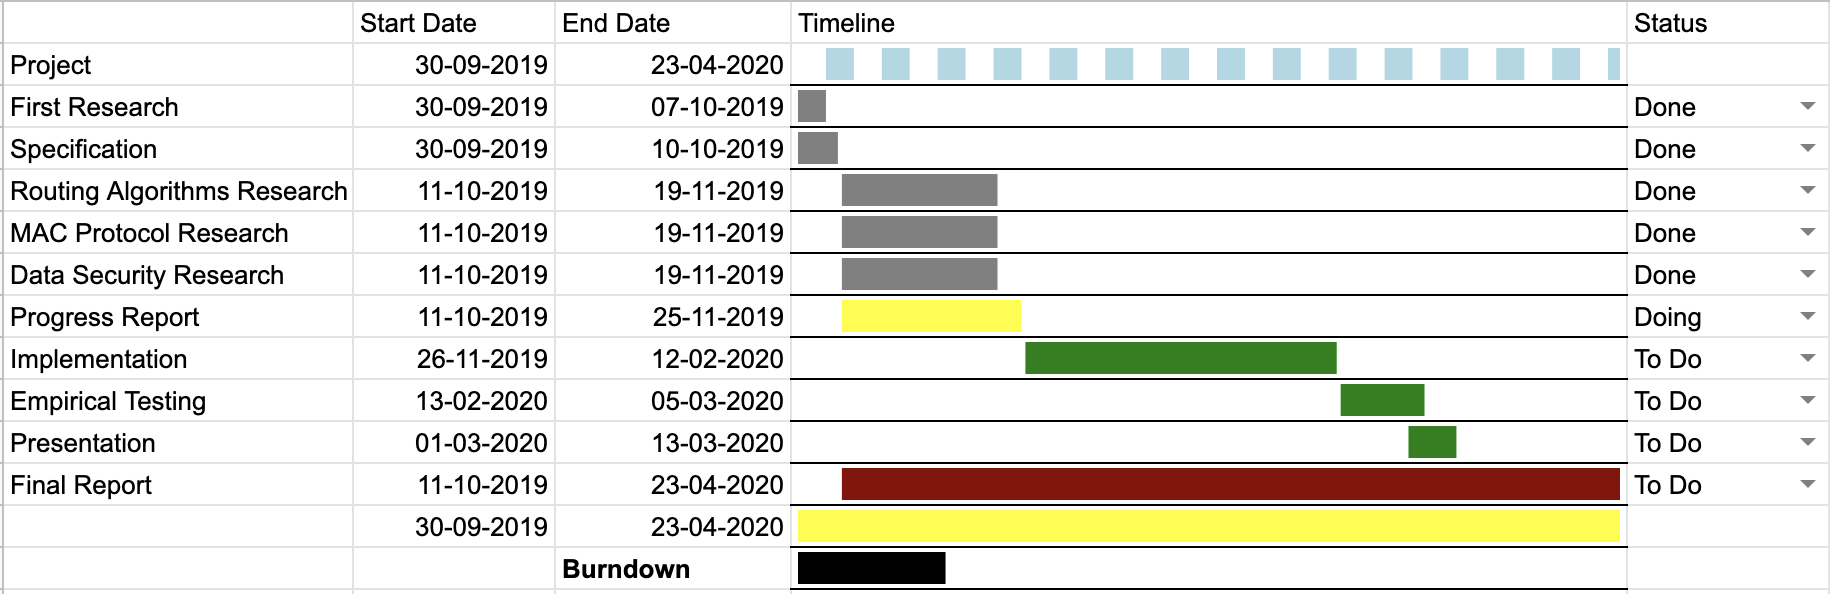
\includegraphics[scale=0.35]{ProjectTimeline}
    \caption{Project Timeline}
    \label{fig:project-timeline}
\end{figure}
\bigskip

As can be seen in fig.\ref{fig:project-timeline}, it shows the predicted project timeline in a Gantt chart as well as displaying the dates between 
which each task will take place. A large block of time 
has been left for the implementation of the project, about 2 months. This gives time for the project code to be written, tested and iterated on. This is to catch bugs and produce a working system. When this is complete, testing of the system will be done to look at the performance of the project so the project can be analysed. With all of this, a presentation will need to be produced. This will detail the different stages of the project, how the system works, as well as retrospectively looking at the project and discussing what went well and what could be improved in the future. With all of this produced, the final report will be written which will discuss all of this in further detail and will assess whether or not the project has been a success. 

\section{Project Tools}

The project will use a variety of tools to accomplish its goals. The project will be written in \textbf{C/C++}. This is because its a low level language and it allows more fine grained control over aspects of the project. Along with this, \textbf{blueZ} will be used to interface with Bluetooth. This is a widely used library for projects such as this, with a number of resources to draw from \cite{huang2007bluetooth}.
\bigskip\\
In terms of hardware, as discussed in the project specification, the project is going to be written for Linux-based devices such as the Raspberry Pi which have 
Bluetooth on-board. Bluetooth is a common technology used by a number of devices, so is a useful medium to use for a project like this. Using a widely used technology increases the number of technologies that this project could apply to. 
\bigskip\\
Other tools are needed to monitor the progress of the project. This project has been using \textbf{Trello} to keep track of tasks which need to be done and have been done. This is being used because its clear to use and allows tasks to be grouped clearly. Alongside this, \textbf{GitHub} has been used to backup code and keep track of project history, in case an older version of the project is needed. This is a widely used product in industry, so is a good choice for this project.

\section{Risk Management}

As mentioned in the project specification, this project doesn't have too many major risks that could have an effect on its performance. One risk, which was discussed above, is losing all physical machines which hold the project. This can be mitigated by storing any code and reports on Github, as well as maintaining a local copy on a hard drive. This provides extra layers of assurance that the project won't be lost. 
\bigskip\\
Another risk is that persons who work on the project fall ill or are unable to do work. This can be mitigated by keeping in contact with DCS and discussing any factors that could lead to a delay in the projects completion because of this reason.
\bigskip\\
Furthermore, there is a risk that part of the project might overrun its planned length of time. This could be because hardware access has been delayed or there are extra technical difficulties that weren't foreseen during the planning of the project. Generous amounts of time have been allowed for each stage, as well as considerations within each stage. For example, in the implementation stage, there are different stages to development. The first stage is to complete basic functionality of the project before layering more features on top. This way of working means there will always be a working version of the project which meets the requirements.

\chapter{Progress}

\section{Defining Project Scope}
The project specification focused on 2 directions for the project, it was quite broad. Since then, the scope of the project has been tightened so that the project is more focused on relevant goals.\\
$\newline$
One option for the project, which was discussed, was a project similar to HIRO-NET \cite{ferranti2019hiro}, a large network which used local bluetooth meshing to pass IP packets to devices, within a piconet/scatternet, which had atleast one active internet connection. With a system like this, routing protocols such as swarm-based routing algorithms \cite{lin2014performance, sharvani2009different, leonov2016modeling} can also be used, enabling further improvements in network efficiency. Some of the benefits of this kind of system are: 
\begin{itemize}
    \item Creates a flexible network 
    \item It is more useful to each survivor as they will have internet access; large variety of services to access
    \item More efficient data efficient; Doesn't constantly flood the network with packets
    \item Easy to implement 2-way communication between survivors and others; Can route packets to and from nodes as network is more stable
\end{itemize}
Although this proposal has a number of huge benefits, it also has a number of drawbacks:
\begin{itemize}
    \item It is difficult to implement and probably beyond the reach of this timeframe. Too much complexity
    \item Difficult to use in a sparsely populated area; Less useful in many environments
    \item May need to use multiple different technologies to accomplish this on top of Bluetooth, such as Wifi. Adds to the already large complexity
    \item Server nodes need to do a lot of work, not good when aiming to conserve battery life
\end{itemize}
An alternative solution is to implement a solution akin to more common DTNs \cite{choksatid2016efficient, wu2011emergency, zhu2012survey, zhu2013relative}, similar to a number of fault-tolerant networks. In this solution, as has been described before, messages about the status of survivors are passed between devices to a sink, usually the emergency services. These messages will contain location data about survivors which can be collected by the emergency services. The packet routing method will be one common to DTNs, either social-based or epidemiology-based. Some of the benefits of this are:
\begin{itemize}
    \item Simple. Makes it easier to implement on a number of different devices so more nodes in the network
    \item Lightweight information. Reduces the packet size so data transmission is quicker
    \item Able to work effectively in both dense and sparse environments
    \item Network focused on emergency services, more beneficial to them
    \item Very tolerant to nodes coming in and out of the network
    \item Works well in topologies with lots of moving nodes
\end{itemize}
Like the first proposal, this also has some issues which have to be considered:
\begin{itemize}
    \item Less efficient. Price of simplicity is that routing is more primitive and so less efficient
    \item 2-way communication is difficult because there is no constant network of devices with addressing
    \item More computation is involved: connections formed with other nodes more often, more nodes routing packets
\end{itemize}
After considering both of these ideas, the direction of the project will be the second proposal, utilising epidemic routing to build a fault-tolerant, lightweight network for spreading information among local, moving nodes. It has a more realistic implementation timetable and has a clearer and better defined use case.  

\section{Timetable}
In the project specification, a timetable was defined which displayed the planned activities which were to be accomplished if the project is to be successful, as well as the dates which they need to be completed by. This was done to give the project structure and to help plan for deadlines. Since this part of the project was submitted, a few changes have been made, as can be seen in fig. \ref{fig:project-timeline}. In this updated timetable, the time for improvements and testing have been rolled into the implementation period. This was done to be in line with principles of test driven development. Also, parts of the timetable have been marked as done. These parts of the project were to be completed in between the project specification and the progress report. These have been completed mostly, as well as some extra research into implementation and working out how the project will work.

\section{Technical}
As well as defining the project scope, work has been done on investigating the technical parts of the project, such as in defining what should be sent within the packets in the network. A principle of the packet structure for the project is that it needs to be small. This is so that as much data as possible can be fit inside as few Bluetooth packets \cite{blepacket} as possible. Only essential information should be included in the packet. Inspirations for a format are the FIX messaging protocol \cite{FIXSPEC}, a widely used protocol for transporting financial data, and JSON \cite{json}, a widely used data format in industry. The advantage of using a protocol like to FIX is that it has a number of security benefits. It uses a group of specified tags which describe very specific information. This means that a program will only analyse the data for specific tags which it cares about, which reduces the chance of unwanted information being processed. If extra functionality is added, nodes can ignore the extra data included, which allows for backwards compatibility in the future. On the otherside, JSON would be good as it is concise and very flexible. There is lots of support for it as it is very established. Both of these offer a lot of inspiration for a format of exchange to use.
\bigskip\\
The data to be included within packets has also been investigated. Obviously, including location data needs to be a priority. This can be done by using GPS, a common way of collecting location data. This is available on most devices today to power a number of location based applications. As well as this, an ID should be included in the packet. This will allow the sink to aggregate the data based on the device from which it originated. As well as this, including a timestamp saying when the packet was generated will allow the sink node to determine how old this data is. This way, it allows the emergency services to determine if the location data is accurate and allows nodes to prioritise which packets to forward first. 
\bigskip\\
As well as considering packets, work has been done working towards understanding how the different libraries work. BlueZ \cite{bluez} is a very useful, and widely used, library for C/C++ but has very little documentation. Much work has been done working towards understanding how it works. As it also contains a number of command line tools, BlueZ has a lot of open source code which uses a lot of the features which this project will use. 

\chapter{Testing}

As discussed in the specification, testing in this project will be used to verify the functionality of the project while changes are made as 
well as being able to verify that requirements have been fulfilled. The project will use different technologies to accomplish this. A unit testing framework will be used, such as \textbf{CUnit}, to test and verify the project. Also, other technologies will be utilised, such as bash scripting. This allows for tests to be written easily for a variety of projects and makes the testing process more flexible.
For integration testing, \textbf{TravisCI} will be used. It is a robust service which is widely used and works very well with GitHub.

\section{Unit Testing}

A test will be written for each part of the project that is written to verify that it functions as it is needed to. Agile development methodologies will be adhered to by writing failing tests, which are then made to be passing by writing the code for which passes the test. Unit testing and its benefits are further discussed in \cite{PressmanUnitIntegration, SommervilleTDD}. 
In these, they discuss the benefits of Test Driven Development and how unit testing works and is beneficial to a project. Unit testing is very useful and allows the functionality of the project to be verified quickly and easily.

\section{Integration Testing}

TravisCI allows larger tests to be written to incorporate more of the project. This is run on a clean VM which 
means there is nothing external to the project which could influence its testing. It enables more rigorous testing and fewer outside influences. This
approach to testing the system is discussed in \cite{PressmanUnitIntegration}.

\section{Success Management}

Success for this project will defined by whether a network of Raspberry Pis, running the software written for this project, can pass packets about their location, between each other to a central repository node representing the emergency services. On top of this, there will be other measures of success for sub-targets, such as data privacy. These targets will be included in the requirements section of this report.


\chapter{Conclusion}
Overall, the project has started smoothly. This part of the project plan has always been earmarked for research into the different areas which the project will touch on. At this stage, a good plan has been developed which will provide a structure for the project going forwards. Obviously, parts of the project will change with implementation, but this is acknowledged in this report. Much of the work which has been done so far has been to define a framework within which the implementation can be done. Being critical, this has been done to a good degree, but some extra work will have to be done during implementation. Not all libraries which will be used have been nailed down and, as a result, how an individual ID will be generated is not 100\% certain yet. Over December, January and much of February, implementation will occur. The project is in a good place to start implementation. Some details are fluid still, but overall much has been nailed down and the majority of research has been completed.

\newpage
\appendix
\addappheadtotoc
\chapter*{Appendices}
\section*{Appendix A}

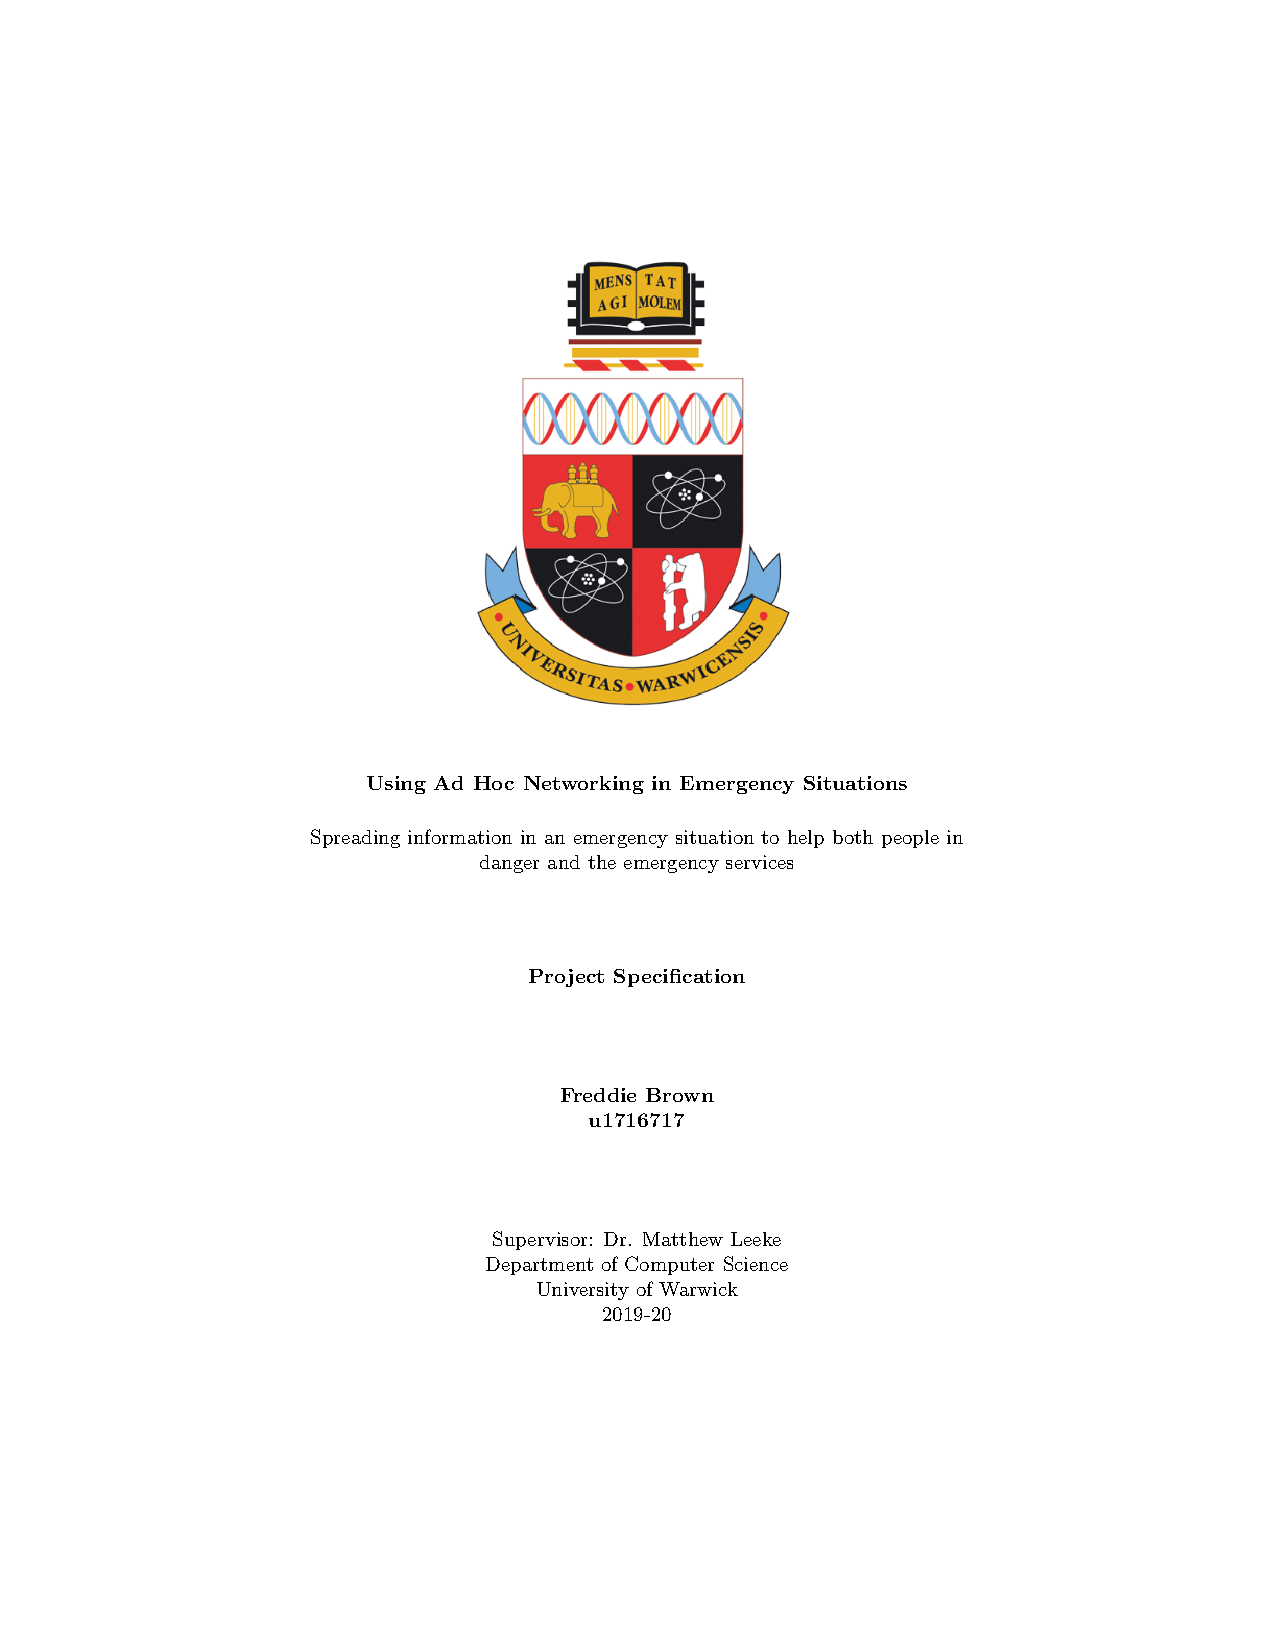
\includepdf[pages={1-20}, fitpaper]{spec.pdf}

\newpage
\addcontentsline{toc}{chapter}{Bibliography}
\bibliography{ref}{}
\bibliographystyle{IEEEtran}

\end{document}
